\documentclass[man,floatsintext]{apa6}
\usepackage{lmodern}
\usepackage{amssymb,amsmath}
\usepackage{ifxetex,ifluatex}
\usepackage{fixltx2e} % provides \textsubscript
\ifnum 0\ifxetex 1\fi\ifluatex 1\fi=0 % if pdftex
  \usepackage[T1]{fontenc}
  \usepackage[utf8]{inputenc}
\else % if luatex or xelatex
  \ifxetex
    \usepackage{mathspec}
  \else
    \usepackage{fontspec}
  \fi
  \defaultfontfeatures{Ligatures=TeX,Scale=MatchLowercase}
\fi
% use upquote if available, for straight quotes in verbatim environments
\IfFileExists{upquote.sty}{\usepackage{upquote}}{}
% use microtype if available
\IfFileExists{microtype.sty}{%
\usepackage{microtype}
\UseMicrotypeSet[protrusion]{basicmath} % disable protrusion for tt fonts
}{}
\usepackage{hyperref}
\hypersetup{unicode=true,
            pdftitle={The Shieh's d and its relation with Cohen's d},
            pdfauthor={Marie Delacre},
            pdfkeywords={keywords},
            pdfborder={0 0 0},
            breaklinks=true}
\urlstyle{same}  % don't use monospace font for urls
\usepackage{graphicx,grffile}
\makeatletter
\def\maxwidth{\ifdim\Gin@nat@width>\linewidth\linewidth\else\Gin@nat@width\fi}
\def\maxheight{\ifdim\Gin@nat@height>\textheight\textheight\else\Gin@nat@height\fi}
\makeatother
% Scale images if necessary, so that they will not overflow the page
% margins by default, and it is still possible to overwrite the defaults
% using explicit options in \includegraphics[width, height, ...]{}
\setkeys{Gin}{width=\maxwidth,height=\maxheight,keepaspectratio}
\IfFileExists{parskip.sty}{%
\usepackage{parskip}
}{% else
\setlength{\parindent}{0pt}
\setlength{\parskip}{6pt plus 2pt minus 1pt}
}
\setlength{\emergencystretch}{3em}  % prevent overfull lines
\providecommand{\tightlist}{%
  \setlength{\itemsep}{0pt}\setlength{\parskip}{0pt}}
\setcounter{secnumdepth}{0}
% Redefines (sub)paragraphs to behave more like sections
\ifx\paragraph\undefined\else
\let\oldparagraph\paragraph
\renewcommand{\paragraph}[1]{\oldparagraph{#1}\mbox{}}
\fi
\ifx\subparagraph\undefined\else
\let\oldsubparagraph\subparagraph
\renewcommand{\subparagraph}[1]{\oldsubparagraph{#1}\mbox{}}
\fi

%%% Use protect on footnotes to avoid problems with footnotes in titles
\let\rmarkdownfootnote\footnote%
\def\footnote{\protect\rmarkdownfootnote}


  \title{The Shieh's d and its relation with Cohen's d}
    \author{Marie Delacre\textsuperscript{1}}
    \date{}
  
\shorttitle{Shieh's d vs Cohen's d}
\affiliation{
\vspace{0.5cm}
\textsuperscript{1} Service of Analysis of the Data, Université Libre de Bruxelles, Belgium}
\keywords{keywords\newline\indent Word count: X}
\usepackage{csquotes}
\usepackage{upgreek}
\captionsetup{font=singlespacing,justification=justified}

\usepackage{longtable}
\usepackage{lscape}
\usepackage{multirow}
\usepackage{tabularx}
\usepackage[flushleft]{threeparttable}
\usepackage{threeparttablex}

\newenvironment{lltable}{\begin{landscape}\begin{center}\begin{ThreePartTable}}{\end{ThreePartTable}\end{center}\end{landscape}}

\makeatletter
\newcommand\LastLTentrywidth{1em}
\newlength\longtablewidth
\setlength{\longtablewidth}{1in}
\newcommand{\getlongtablewidth}{\begingroup \ifcsname LT@\roman{LT@tables}\endcsname \global\longtablewidth=0pt \renewcommand{\LT@entry}[2]{\global\advance\longtablewidth by ##2\relax\gdef\LastLTentrywidth{##2}}\@nameuse{LT@\roman{LT@tables}} \fi \endgroup}


\usepackage{lineno}

\linenumbers

\authornote{

Correspondence concerning this article should be addressed to Marie Delacre, CP191, avenue F.D. Roosevelt 50, 1050 Bruxelles. E-mail: \href{mailto:marie.delacre@ulb.ac.be}{\nolinkurl{marie.delacre@ulb.ac.be}}}

\abstract{

}

\begin{document}
\maketitle

Unlike the classical Cohen's \(\delta\), Shieh's \(\delta\) depends on the sample size ratio (that I will call later nratio). For the same amount of differences betweeen two means, same standard deviations (sd) and sd-ratio, Shieh's \(\delta\) will vary as a function of the nratio. To illustrate the relation between Shieh's \(\delta\) and the nratio, we can calculate the parameter across a range of nratio. We will first study the Shieh's \(\delta\) (and its relation with Cohen's \(\delta\)) when variances are equal between groups. We will then go through the relation when variances are unequal between groups.

\hypertarget{when-variances-are-equal-between-groups}{%
\section{When variances are equal between groups}\label{when-variances-are-equal-between-groups}}

As a first example, in Figure \ref{fig:SHIEH1}, Cohen's \(\delta\) and Shieh's \(\delta\) are calculated for different configurations where the observed mean difference (\(\mu_{1}-\mu_{2}\)) is 1, the total sample size is 200 and standard deviation of each groups \(\sigma_{1}\) and \(\sigma_{2}\) both equals 2. As one can see, as long as variances are equal between groups, Cohen's \(\delta\) remains constant for all nratio, unlike Shieh's \(\delta\). Moreover, Shieh's \(\delta\) achieves its maximum value when \(n_{1}\) = \(n_{2}\) (in Figure \ref{fig:SHIEH1}, Shieh's \(\delta\) equals 0.25 when nratio is 1). One can also see that at the maximum point value, the relation between Shieh's \(\delta\) and Cohen's \(\delta\) is as follows:

\begin{equation} 
\hat{\delta}_{Cohen}=2 \times \hat{\delta}_{Shieh}  
\label{eq:cohenshieh}
\end{equation}

\begin{figure}
\centering
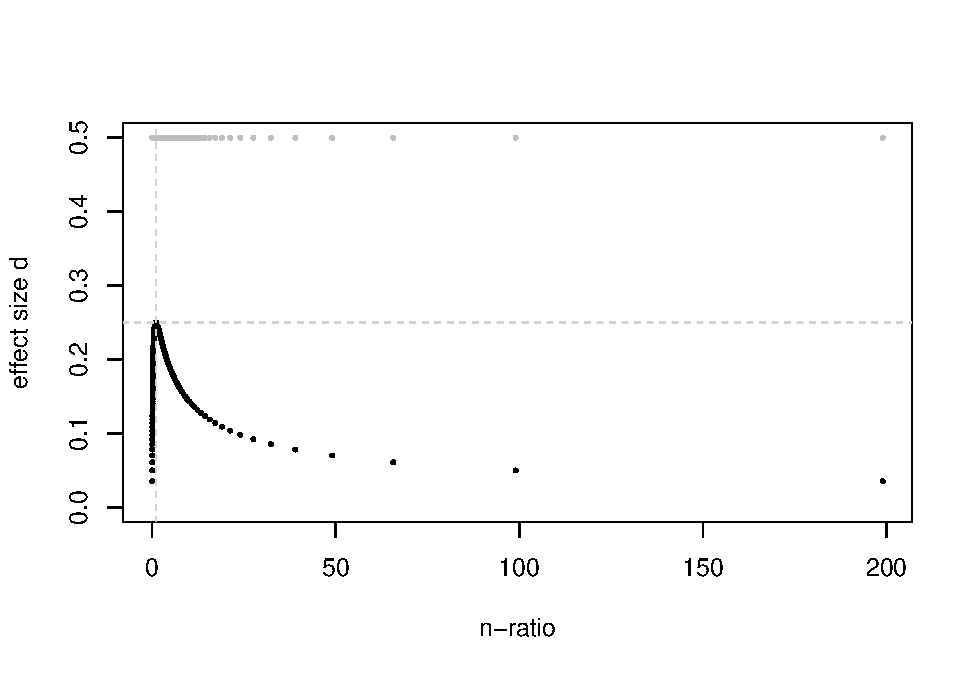
\includegraphics{The-shieh-s-and-its-relation-with-Cohen-s-d_files/figure-latex/SHIEH1-1.pdf}
\caption{\label{fig:SHIEH1}Comparison of Shieh's d (black dots) and Cohen's d (grey dots) when mu1 - mu2 = 1, N = 200 and sigma 1 and sigma 2 both equals 2}
\end{figure}

When plotting both parameters against the log of the nratio, one can more easily observe that the Shieh's \(\delta\) departs symmetrically from it's maximum value as long as the nratio moves away from 1 (see Figure \ref{fig:SHIEH2}). The relation between all Shieh's \(\delta\) values and its value when nratio=1 can be expressed as follows:

\begin{equation} 
max(\hat{\delta}_{Shieh})= \hat{\delta}_{Shieh} \times \frac{nratio+1}{2 \times sqrt(nratio)}
\label{eq:shiehvsmax}
\end{equation}

Because we know from \eqref{eq:cohenshieh} than \(max(\hat{\delta}_{Shieh})\) is half of the value of \(\hat{\delta}_{Cohen}\), we can therefore deduce a more general relation between Cohen's \(\delta\) and Shieh's \(\delta\):

\begin{equation} 
\hat{\delta}_{Cohen}= \hat{\delta}_{Shieh} \times \frac{nratio+1}{sqrt(nratio)}
\label{eq:cohenshiehgen}
\end{equation}

This relations remains true as long as variances are equal between groups.

\begin{figure}
\centering
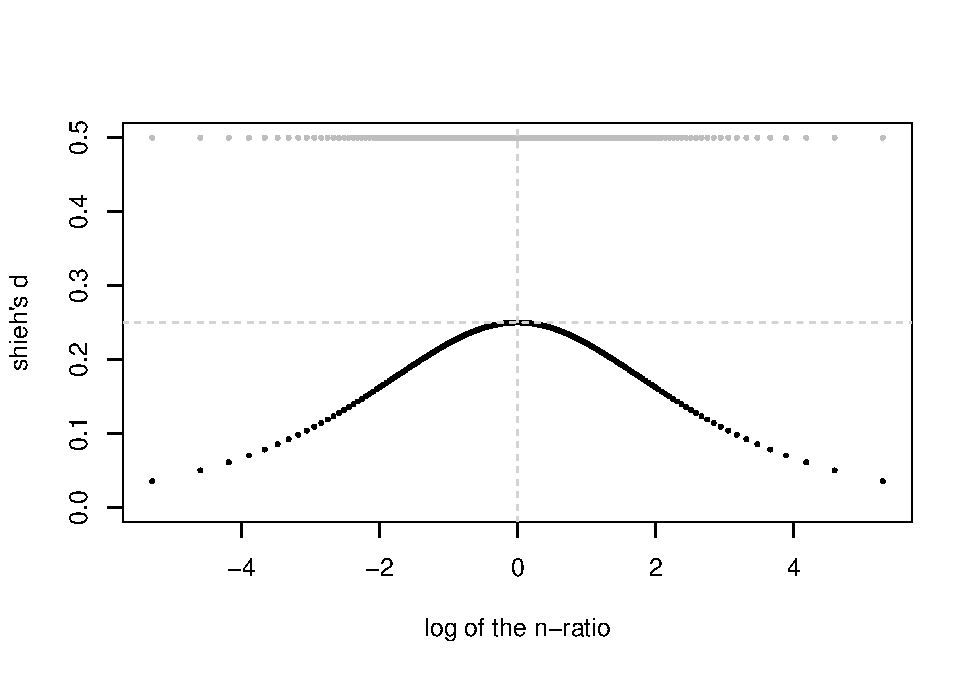
\includegraphics{The-shieh-s-and-its-relation-with-Cohen-s-d_files/figure-latex/SHIEH2-1.pdf}
\caption{\label{fig:SHIEH2}Comparison of Comparison of Shieh's d (black dots) and Cohen's d (grey dots) when mu1 - mu2 = 1, N = 200 and delta 1 = delta 2 = 2}
\end{figure}

\hypertarget{when-variances-are-unequal-between-groups}{%
\section{When variances are unequal between groups}\label{when-variances-are-unequal-between-groups}}


\end{document}
